Following the initial validation of gelatine as a conductive medium through the cube prototypes, the next step in the development process involved assembling a full-scale homogeneous phantom head model. For this purpose, the Open EEG Phantom design~\cite{OpenEEGPhantom} was selected, an open-source head model available through the Open Science Framework repository. This model provides a standardized geometry for \gls{eeg} phantom testing and has been documented for reproducibility in research applications.

The assembly process followed the fabrication protocol described in the repository documentation, utilizing a gelatine-based conductive medium to fill the head-shaped mold. The printed model and its assembly are illustrated in Figures~\ref{fig:open_eeg} and~\ref{fig:open_eeg_2} respectively.

\begin{figure}[H]
    \centering
    \begin{subfigure}[b]{0.6\textwidth}
        \centering
        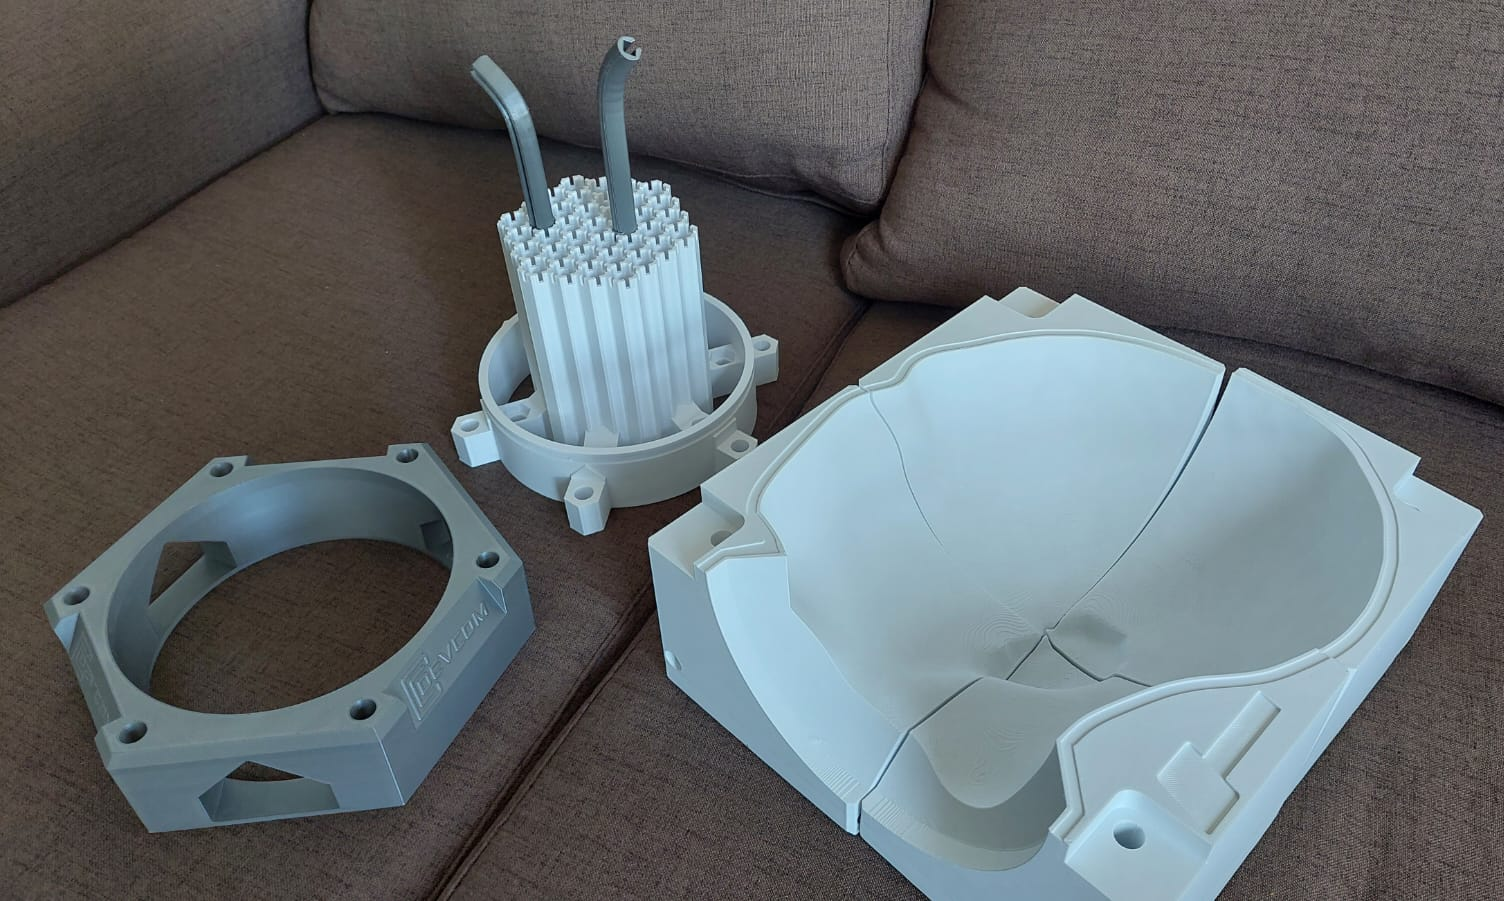
\includegraphics[height=6cm]{../../02_Images/open_eeg.png}
        \caption{Open EEG Phantom 3D printed parts}%
        \label{fig:head_overview_complete}
    \end{subfigure}
    % \hfill
    \begin{subfigure}[b]{0.35\textwidth}
        \centering
        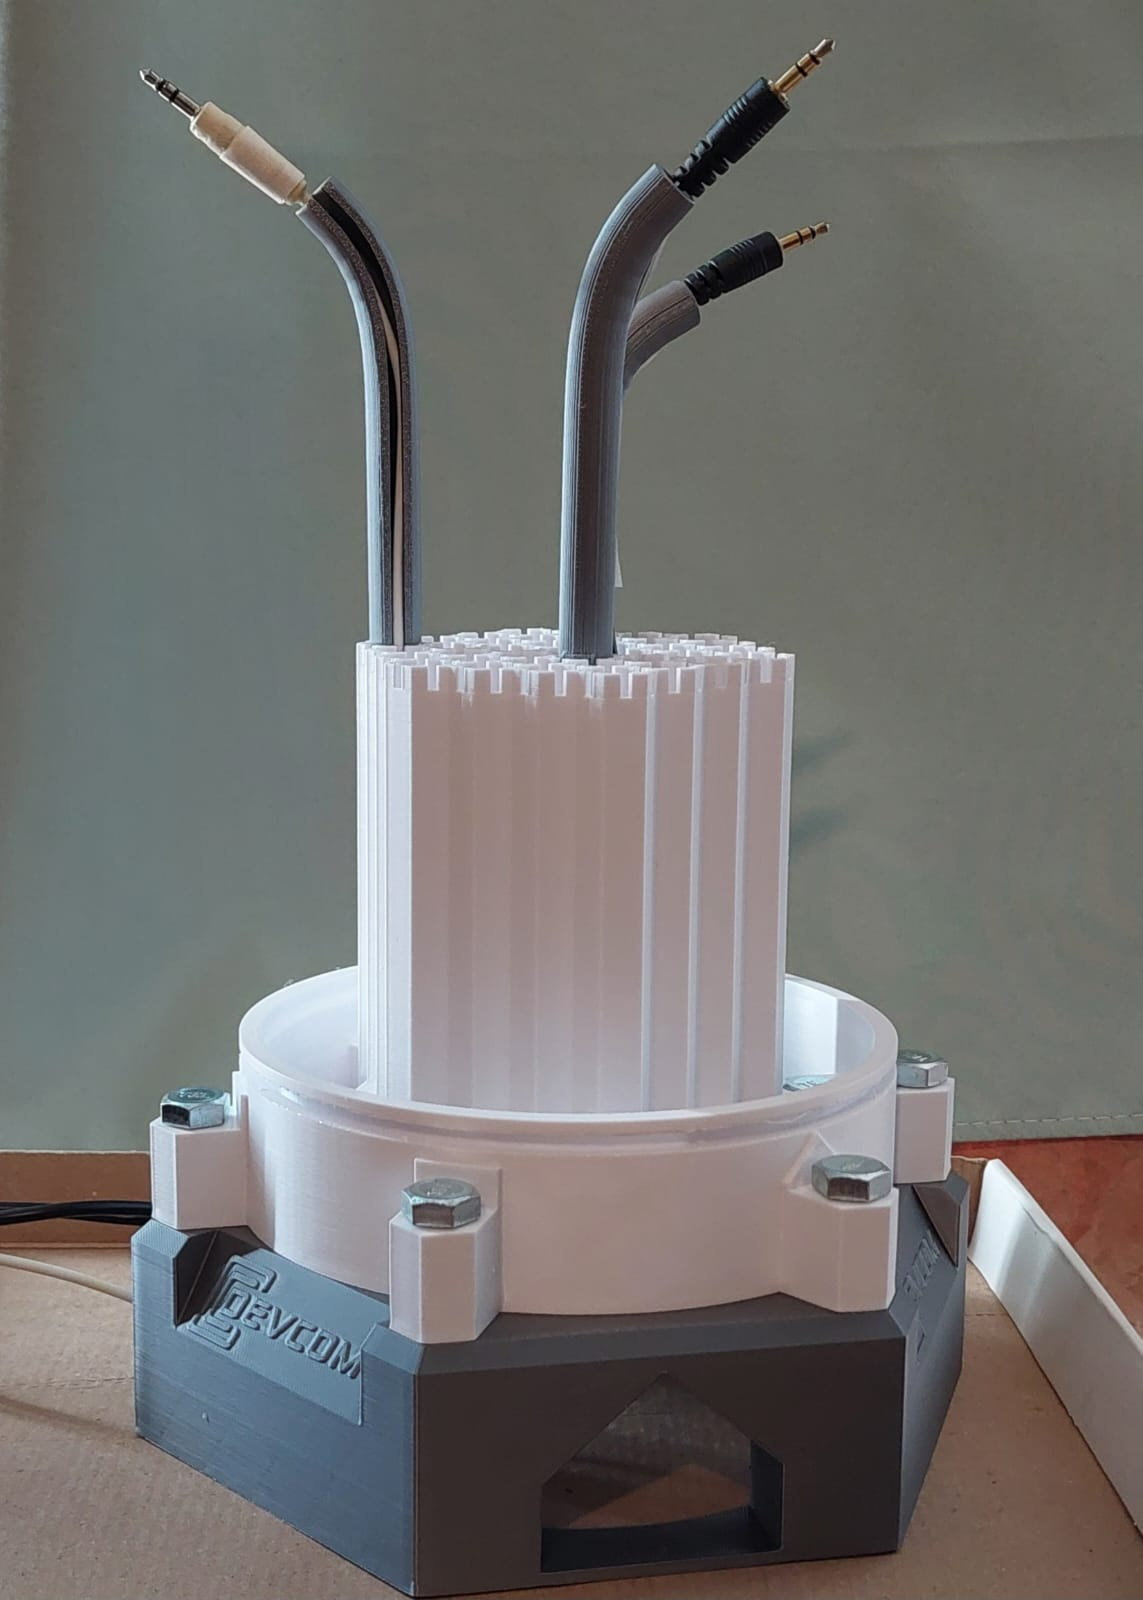
\includegraphics[height=6cm]{../../02_Images/open_eeg_2.jpeg}
        \caption{Open EEG Phantom internal structure}%
        \label{fig:head_overview_section}
    \end{subfigure}
    \caption[Open EEG Phantom 3D model]{3D model of the Open EEG phantom head, highlighting major components and internal structure.}%
    \label{fig:open_eeg}
\end{figure}

\begin{figure}[H]
    \centering
    \begin{subfigure}[b]{0.45\textwidth}
        \centering
        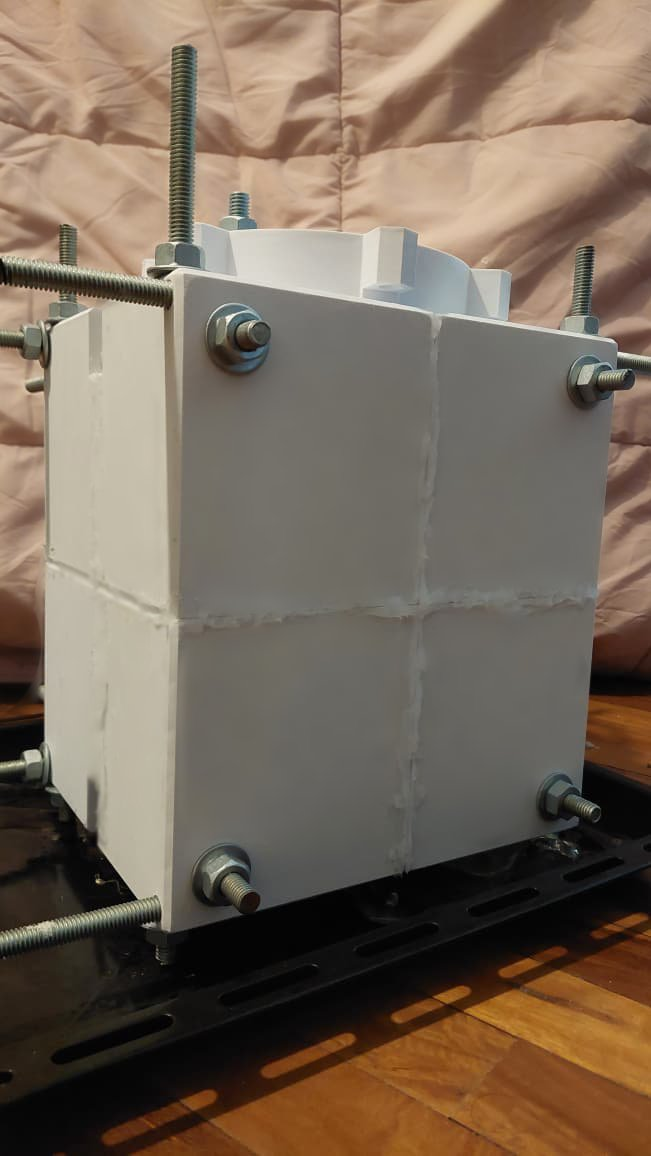
\includegraphics[height=9cm]{../../02_Images/open_phantom_assembly.jpeg}
        \caption{Side view}%
        \label{fig:open_phantom_assembly}
    \end{subfigure}
    % \hfill
    \begin{subfigure}[b]{0.45\textwidth}
        \centering
        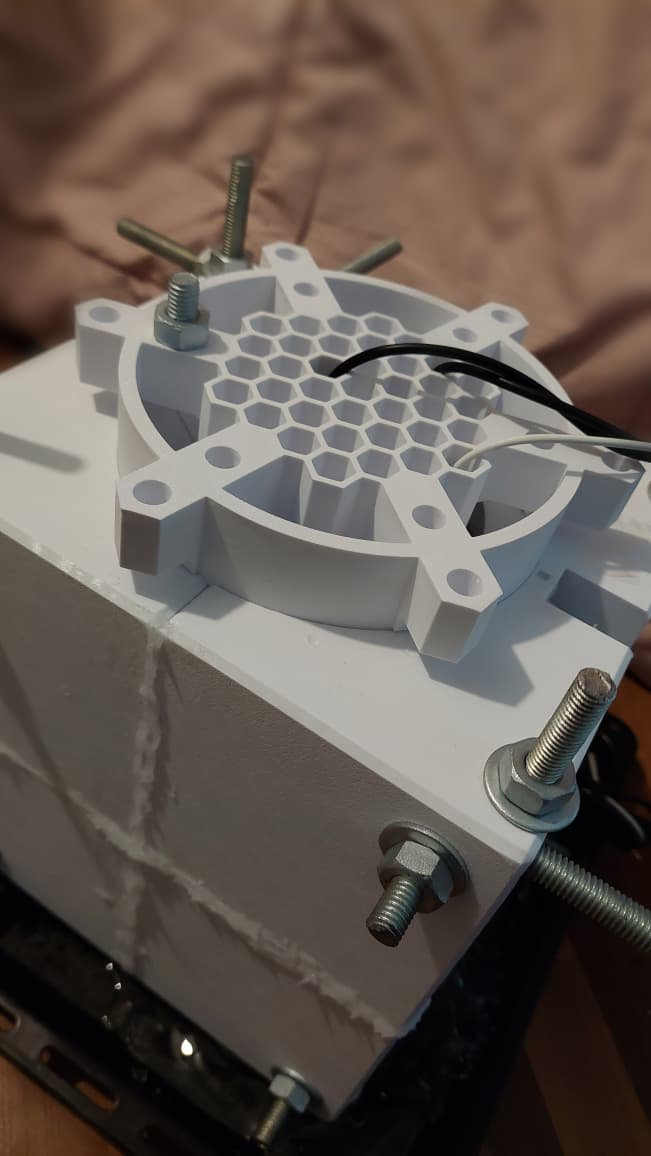
\includegraphics[height=9cm]{../../02_Images/open_phantom_assembly_2.jpeg}
        \caption{Top view}%
        \label{fig:open_phantom_assembly_2}
    \end{subfigure}
    \caption[Open EEG Phantom Assembly]{Assembly of the Open EEG Phantom head model using gelatine as the conductive medium.}%
    \label{fig:open_eeg_2}
\end{figure}